\documentclass[
	letterpaper, % Paper size, specify a4paper (A4) or letterpaper (US letter)
	10pt, % Default font size, specify 10pt, 11pt or 12pt
]{CSUniSchoolLabReport}

%----------------------------------------------------------------------------------------
%	REPORT INFORMATION
%----------------------------------------------------------------------------------------

\title{Frequency Content of Signals\\ Circuits \& Signals \\ EECE2150} % Report title

\author{Michael \textsc{Brodskiy}}

\date{March 27, 2023} % Date of the report

%----------------------------------------------------------------------------------------


\begin{document}

\maketitle % Insert the title, author and date using the information specified above

\begin{center}
	\begin{tabular}{l r}
		Date Performed: & March 16, 2023 \\ % Date the experiment was performed
        Partner: & Juan \textsc{Zapata} \\ % Partner names
		Instructor: & Professor \textsc{Sun} % Instructor/supervisor
	\end{tabular}
\end{center}

\setcounter{section}{-1}

\section{Introduction}

The purpose of this laboratory experimentation was to demonstrate signal analysis through fast Fourier transforms, as well as connecting this concept to real-world signals. In the case of this lab, the real-world signals used were that of voice recordings, which demonstrate Fourier response to different sounds.

\section{Discussion and Analysis}

\subsection{Q1} The highest peak in the spoken audio signal occurs at $100[\si{\hertz}]$. There are subsequent peaks at $200[\si{\hertz}]$, $350[\si{\hertz}]$, and $500[\si{\hertz}]$. Most of the signal is between $0$ and $600[\si{\hertz}]$. There is a smaller peak at $4300[\si{\hertz}]$. (Shown in Figure \ref{fig:1})

\begin{figure}[H]
  \centering
  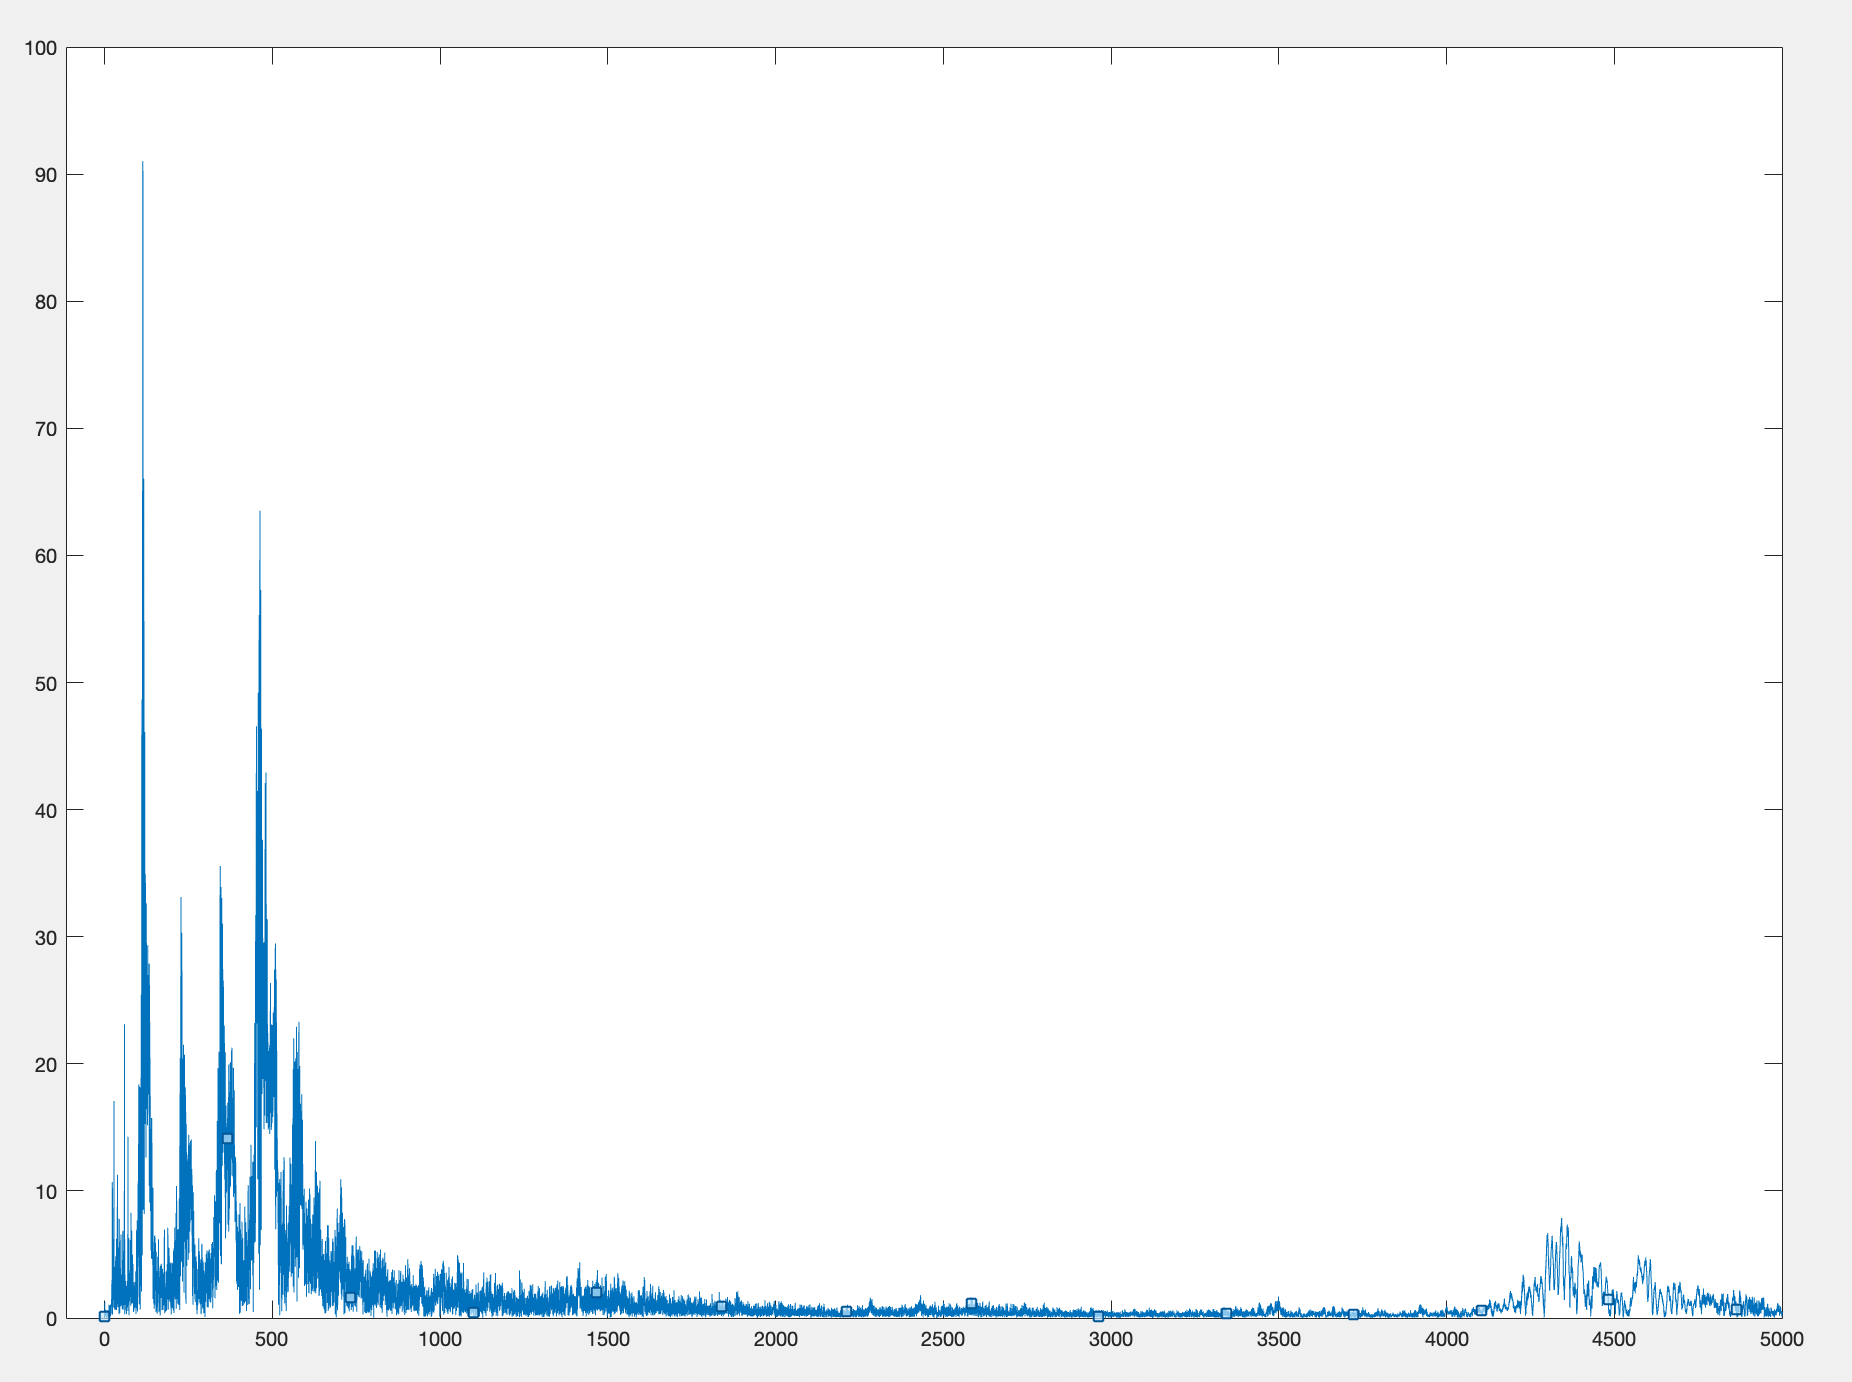
\includegraphics[width=.9\textwidth]{Figures/L12Q1.png}
  \caption{The Generated Fourier Analysis}
  \label{fig:1}
\end{figure}

\subsection{Q2} The frequency almost never goes past $500[\si{\hertz}]$. What changes is the amplitude of these frequencies in different subintervals. (Shown in Figures \ref{fig:2}-\ref{fig:4})

\begin{figure}[H]
  \centering
  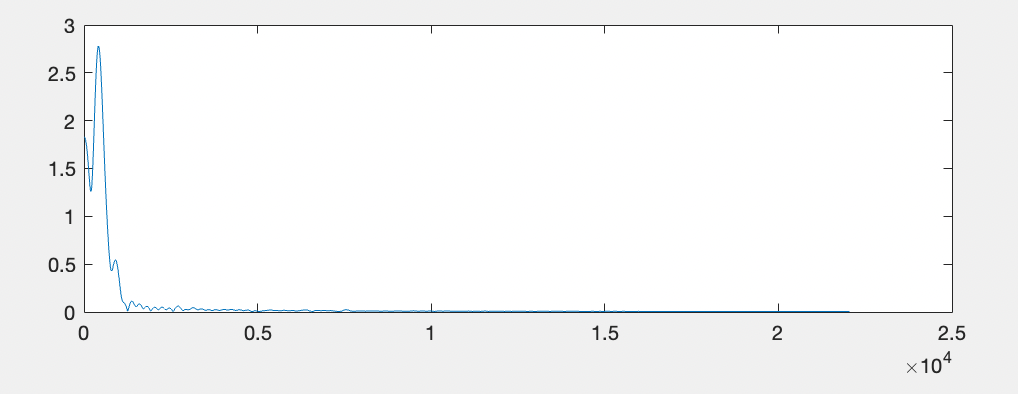
\includegraphics[width=.9\textwidth]{Figures/L12Q2-1.png}
  \caption{Subinterval One}
  \label{fig:2}
\end{figure}

\begin{figure}[H]
  \centering
  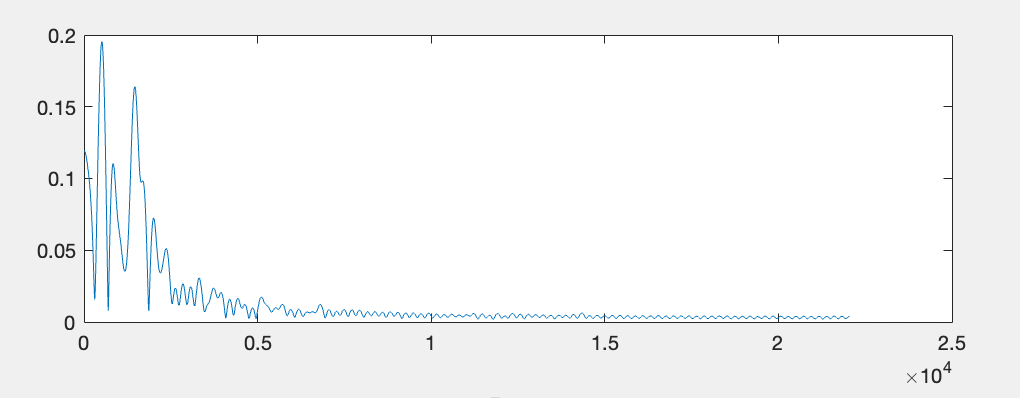
\includegraphics[width=.9\textwidth]{Figures/L12Q2-2.png}
  \caption{Subinterval Two}
  \label{fig:3}
\end{figure}

\begin{figure}[H]
  \centering
  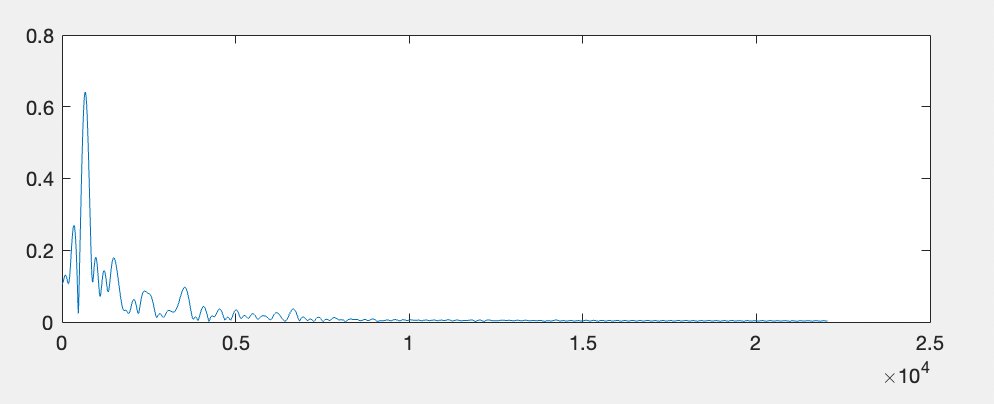
\includegraphics[width=.9\textwidth]{Figures/L12Q2-3.png}
  \caption{Subinterval Three}
  \label{fig:4}
\end{figure}

\subsection{Q3} Using a vowel sound, spikes were produced, as well as other harmonically-related spikes. The tallest spike is at $115[\si{\hertz}]$. There are other spikes at 230, 345, 460, 575, 690, 805, and $920[\si{\hertz}]$. The height of the spikes decrease as the frequency increases, except at $575[\si{\hertz}]$. (Shown in Figure \ref{fig:5})

\begin{figure}[H]
  \centering
  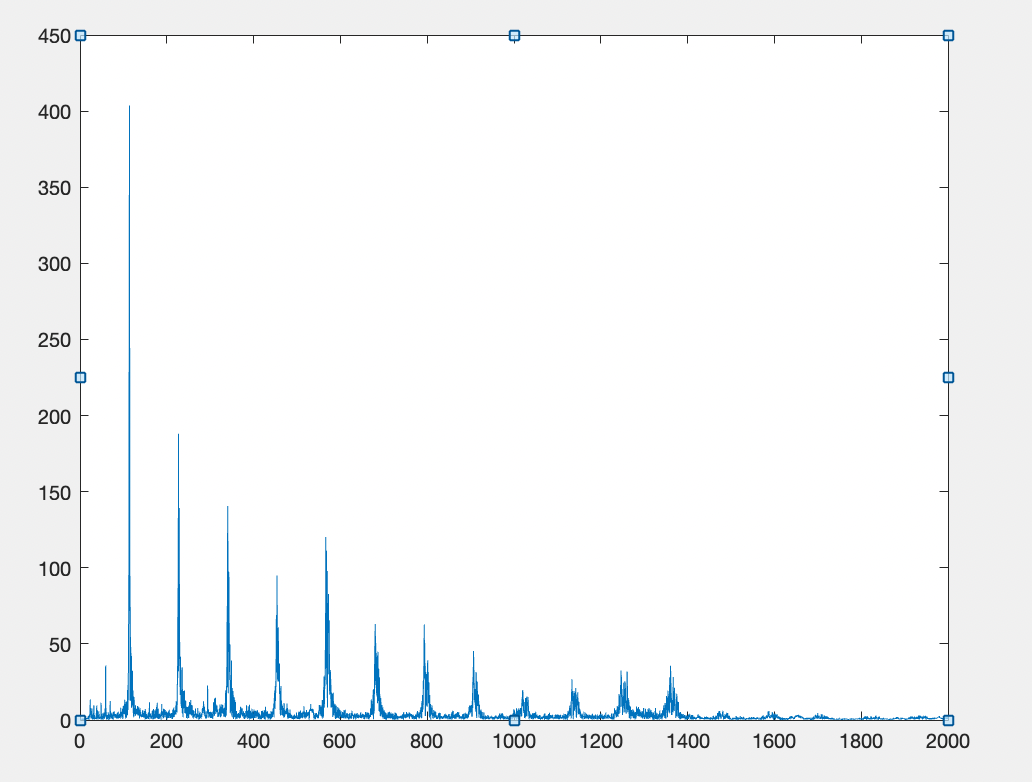
\includegraphics[width=.9\textwidth]{Figures/L12Q3.png}
  \caption{Fourier Transform Using Vowels}
  \label{fig:5}
\end{figure}

\subsection{Q4} Making a sound like `\textsc{sh}' produces more frequencies than a constant vowel sound. It has a control spike at $300[\si{\hertz}]$, and it has a relatively high amplitude at most frequencies in the range of $0$-$600[\si{\hertz}]$. (Shown in Figure \ref{fig:6})

\begin{figure}[H]
  \centering
  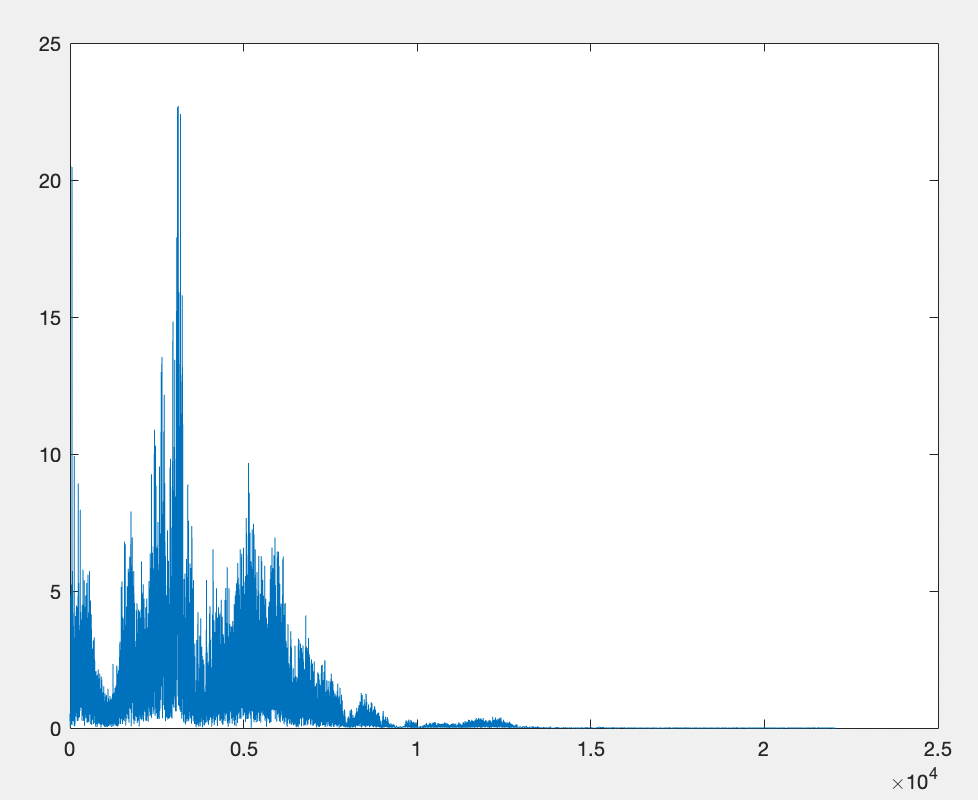
\includegraphics[width=.9\textwidth]{Figures/L12Q4.png}
  \caption{Fourier Transform Using `\textsc{Shh}' Sound}
  \label{fig:6}
\end{figure}

\subsection{Q5} There are slight differences between the two peoples' spectra.

\subsection{Q6} For both signals, the range with the dominant frequency content is $0$-$60[\si{\hertz}]$. (Shown in Figures \ref{fig:7}-\ref{fig:8})

\begin{figure}[H]
  \centering
  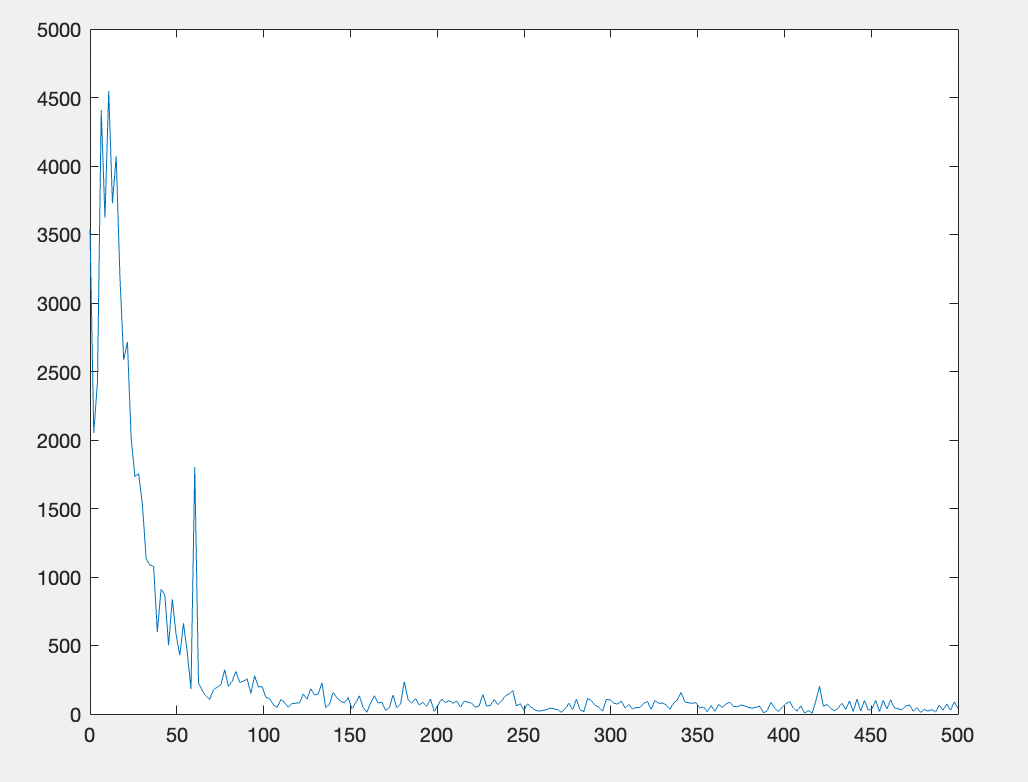
\includegraphics[width=.9\textwidth]{Figures/L12Q6-1.png}
  \caption{ECG1 Waveform}
  \label{fig:7}
\end{figure}

\begin{figure}[H]
  \centering
  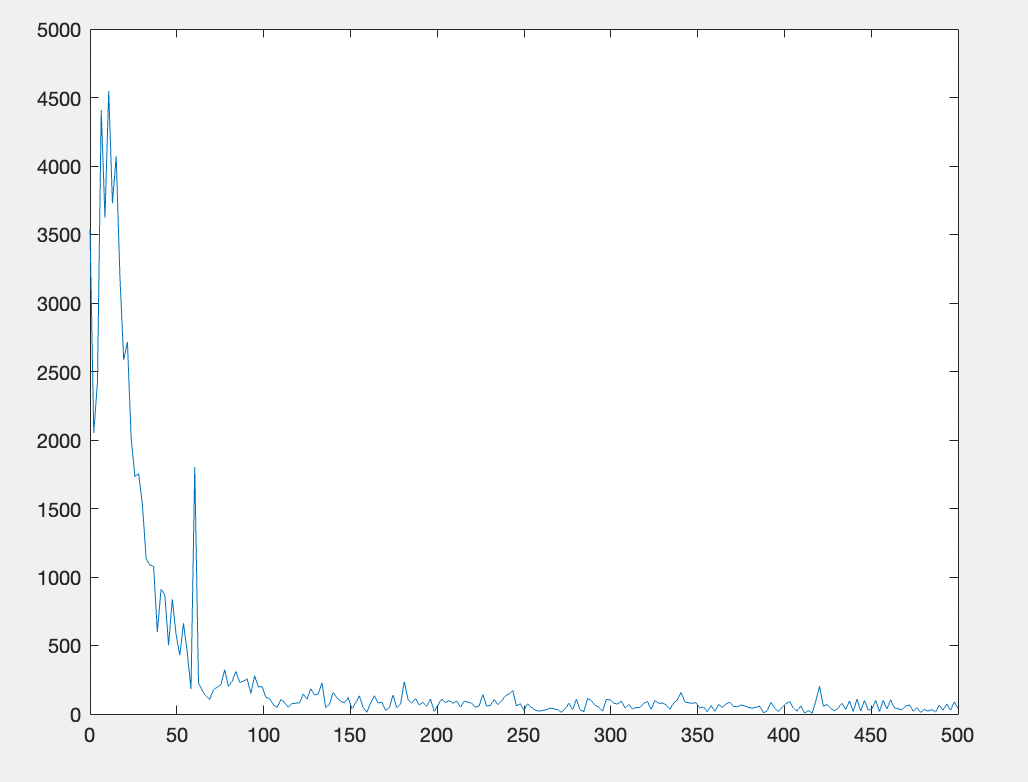
\includegraphics[width=.9\textwidth]{Figures/L12Q6-1.png}
  \caption{ECG2 Waveform}
  \label{fig:8}
\end{figure}

\subsection{Q7} The frequency of the major noise content in ECG1 is $60[\si{\hertz}]$

\subsection{Q8} The highest peak is at $1.25[\si{\hertz}]$. At a rate of $1.25[\si{\hertz}]\cdot60=75[\text{bpm}]$

\subsection{Q9} There is no noticeable additional noise in either signal.

\subsection{Q10} I would want to amplify the frequencies from $0$-$50[\si{\hertz}]$, and reject anything above $100[\si{\hertz}]$

\subsection{Q11} At least $200[\si{\hertz}]$ sampling rate, as this allows up to $200[\si{\hertz}]$ of the signal

\section{Conclusion}

Overall, this laboratory experiment allowed for a thorough analysis of real-world signals through the use of Fourier transforms. By applying this somewhat abstract topic to real life scenarios, the concept of the Fourier transform becomes much easier to grasp.

\end{document}
